\chapter{ORB SLAM}

\section{特征提取--ORBextractor}


\begin{figure}[h]%%图
	\centering  %插入的图片居中表示
	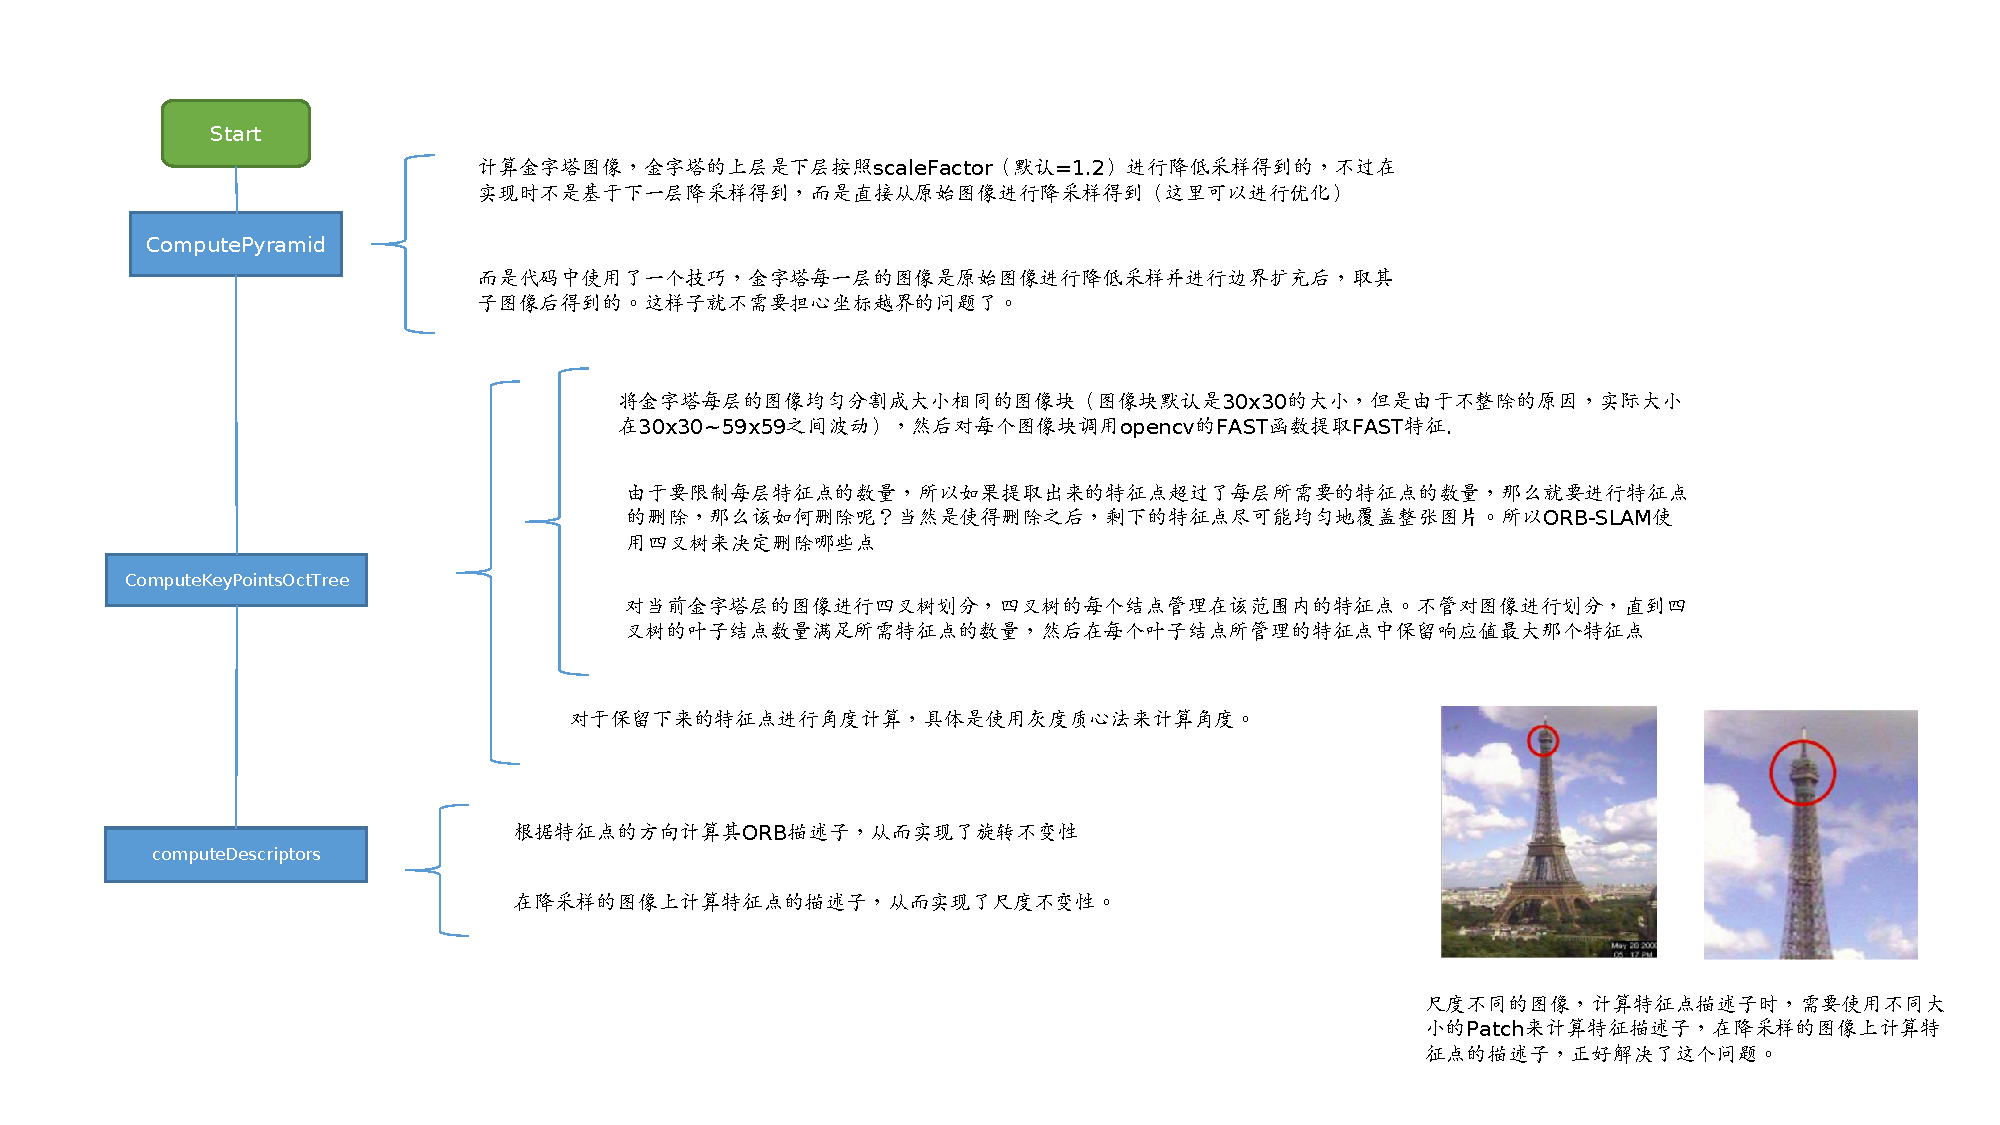
\includegraphics[width=1.0\linewidth]{image/ORB-SLAM/ORBextractor.pdf}  %插入的图,包括JPG,PNG,PDF,EPS等,放在源文件目录下
	\caption{ORB特征提取流程图.}  %图片的名称
	\label{fig:orb_extractor}   %标签,用作引用
\end{figure}


下面是ORB-SLAM构造金字塔的代码:
\begin{lstlisting}[language = C++]
void ORBextractor::ComputePyramid(cv::Mat image)
{
	for (int level = 0; level < nlevels; ++level)
	{
		float scale = mvInvScaleFactor[level];
		// 这是根据尺度进行降采样之后的图像大小
		Size sz(cvRound((float)image.cols*scale), cvRound((float)image.rows*scale));
		// 这是在降采样之后的图像上加上边界之后的大小
		Size wholeSize(sz.width + EDGE_THRESHOLD*2, sz.height + EDGE_THRESHOLD*2);
		Mat temp(wholeSize, image.type()), masktemp;
		// 将temp中的图像部分,非边界部分,赋值到mvImagePyramid
		mvImagePyramid[level] = temp(Rect(EDGE_THRESHOLD, EDGE_THRESHOLD, sz.width, sz.height));
		
		// Compute the resized image
		if( level != 0 )
		{
			resize(mvImagePyramid[level-1], mvImagePyramid[level], sz, 0, 0, INTER_LINEAR);
			
			copyMakeBorder(mvImagePyramid[level], temp, EDGE_THRESHOLD, EDGE_THRESHOLD, EDGE_THRESHOLD, EDGE_THRESHOLD,
			BORDER_REFLECT_101+BORDER_ISOLATED);            
		}
		else
		{
			copyMakeBorder(image, temp, EDGE_THRESHOLD, EDGE_THRESHOLD, EDGE_THRESHOLD, EDGE_THRESHOLD,
			BORDER_REFLECT_101);            
		}
	}
	
}
\end{lstlisting}
ORB-SLAM在构造金字塔时用到了一个技巧,其中\textbf{sz}是降采样之后的图像大小;\textbf{wholeSize}是降采样之后的图像加上边界之后的大小;图像temp的大小是\textbf{wholeSize},接着将图像temp的非边界部分(降采样的图像区域,此时该区域还没有内容)赋值给mvImagePyramid,之后计算ORB特征点时,用到的是mvImagePyramid,哪怕其坐标越界(不要越界太多),那么都是没有问题的。




ORB-SLAM在计算特征点角度时,使用了灰度质心法。需要注意的是,其使用的是圆形patch来计算方向的,所以就必须要知道圆形patch的每一行有多长。ORBextractor在初始化的时候就预计算了圆形patch的每一行有多长(实际上是每一行长度的一半)并存储在umax数组中。



\section{特征匹配--ORBmatcher}

ORBMatcher中的匹配大致分为两种:一种是图像帧知道位姿的匹配;另一种是图像帧不知道位姿的匹配。

\begin{enumerate}
	\item \textbf{已知图像帧位姿的特征点匹配}:因为已知图像帧位姿,所以能够3D点投影到该图像帧上,然后在投影点的周围搜索匹配,从而得到2D-3D点匹配。
	\item \textbf{未知图像帧位状的特征点匹配}:如果不知道图像位姿,那么则使用BoW向量来进行匹配,实际上是通过DBoW2得到的FeatureVector来快速计算特征点之间的匹配。由于正确的特征点匹配一般在Vocabulary Tree上是属于同一个结点的,所以只需要在两张图像帧上,在属于同一个结点的特征点之间进行匹配。
\end{enumerate}

上面的两种匹配策略,都限制了每个特征点所需要测试的特征点数量,从而提高了特征点匹配的效率。




\section{帧间追踪--Tracking线程}

Tracking线程的流程如图\ref{fig:orb_tracking}所示。

\begin{figure}[h]%%图
	\centering  %插入的图片居中表示
	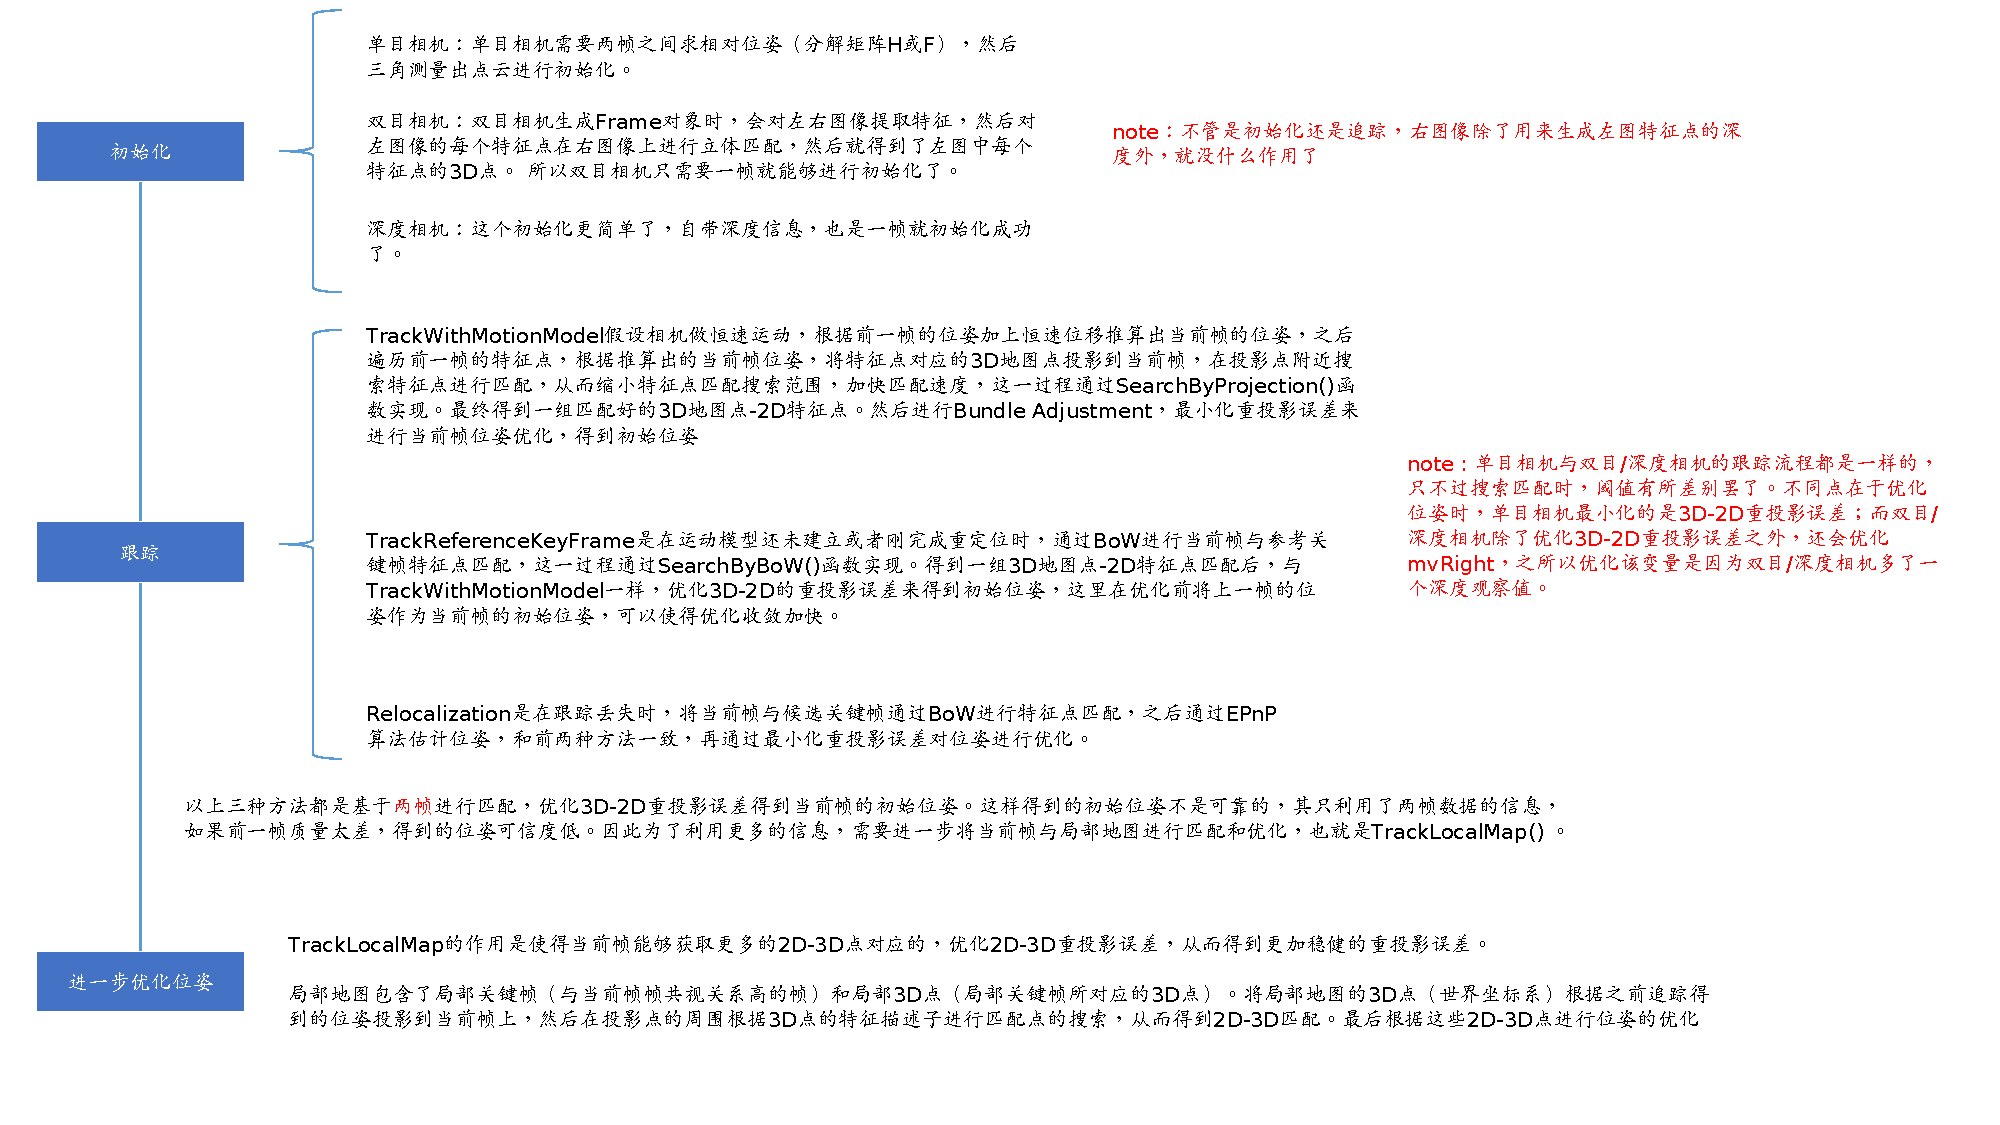
\includegraphics[width=1.0\linewidth]{image/ORB-SLAM/Tracking.pdf}  %插入的图,包括JPG,PNG,PDF,EPS等,放在源文件目录下
	\caption{帧间跟踪流程图.}  %图片的名称
	\label{fig:orb_tracking}   %标签,用作引用
\end{figure}





\section{局部建图--LocalMapping线程}

ORB-SLAM2中的LocalMapping线程是用来对\textbf{关键帧}进行建图的,也即尽可能恢复关键帧中2D特征点所对应的3D点的坐标,其流程如图\ref{fig:local_mapping}所示。

Tracking线程会将创建好的关键帧插入到LocalMapping线程的队列中,而LocalMapping线程要做的就是不断取出队列中的关键帧,对其进行建图。

\begin{enumerate}
	\item LocalMapping取出队首第一帧之后,先是处理该关键帧已有的2D-3D对应关系(追踪该关键帧时,所得到的2D-3D点对应关系),其实就是将2D点添加为3D点的观测;
	\item 然后就是删除一些不稳定、或是错误的3D点,LocalMapping线程会维护一个mlpRecentAddedMapPoings列表,该列表存储了一些最近新三角测量得到的3D点,在经过一段时间后,如果某些3D点的observation数量太少的话,那么就说明该3D点不稳定、或者是错误的,则会被删除;
	\item 接着就是对该关键帧上那些没有3D点对应的2D点进行三角测量了,对于没有3D点对应的2D点在该关键帧的相邻关键帧上寻找匹配点(利用BoW寻找匹配),对于找到的匹配点进行极线验证,对于通过极线验证的2D-2D匹配点才会进行三角测量,对于单目相机,肯定是进行三角测量,而对于双目/深度相机,则有可能使用其自带的深度信息而不进行三角测量。得到3D点后,还需要进行一系列的检测才会决定创不创建该3D点为MapPoint,具体的条件为深度在两帧图像上为正,在两帧图像上的重投影误差不能太大等。
	\item 在创建完新的3D点之后,如果当前线程空闲(也即关键帧队列为空),那么就进行3D点的融合处理。因为ORB-SLAM2进行的是\textbf{二视图三角测量},而一个3D点的观测(2D点)可能会出现在很多张图像上,这样子就会导致三角测量出多个3D点,3D点融合要做的就是让这些2D点(观测)变成同一个3D点的observation。\begin{enumerate}[(1)]
		\item 将当前关键帧的3D点投影到其相邻关键帧上,然后在一定的半径内找到2D匹配点(找到特征描述子距离最小的匹配点,并且该距离要小于阈值,因为距离最小并不代表就是匹配点,因此还要判断距离阈值)进行融合。融合的方法是:(a)如果该2D点没有3D点对应,那么就让该2D点称为当前关键帧3D点的observation;(b)如有该2D点存在3D点对应,那么现在就有了两个3D点了,根据哪个3D点的observation多(稳定),那么就以哪个3D点为准,并且融合两个3D点的observation。
		\item 将相邻关键帧的3D点投影到当前关键帧,然后找到匹配点,进行融合。
		\end{enumerate}
	\item 最后,删除冗余的关键帧。如果该关键帧90\%的3D点都能在其某个相邻关键帧上看到,那么就认为该关键帧是冗余的,可以删除。

\end{enumerate}



\begin{figure}[h]%%图
	\centering  %插入的图片居中表示
	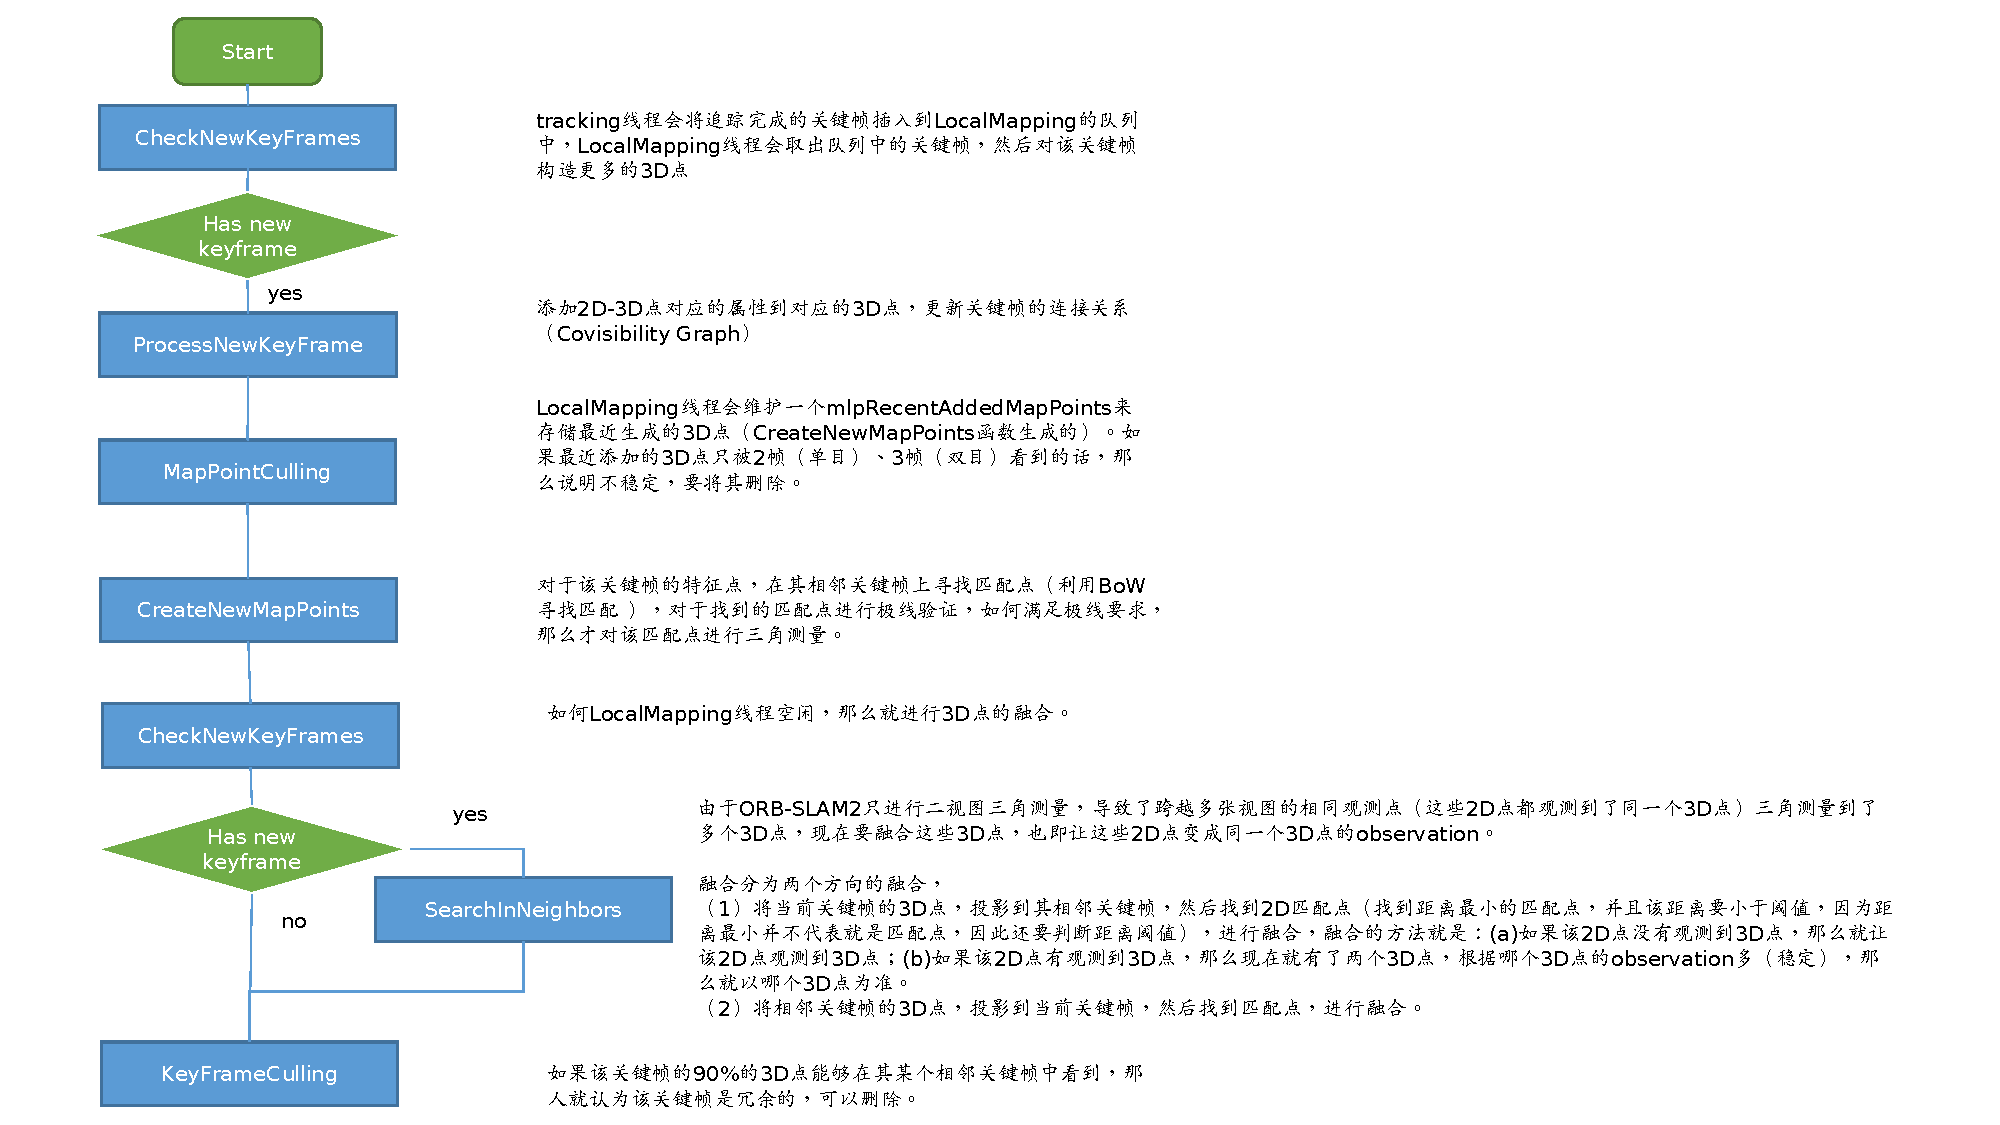
\includegraphics[width=1.0\linewidth]{image/ORB-SLAM/LocalMapping.pdf}  %插入的图,包括JPG,PNG,PDF,EPS等,放在源文件目录下
	\caption{ORB-SLAM2局部建图流程图.}  %图片的名称
	\label{fig:local_mapping}   %标签,用作引用
\end{figure}





\section{闭环修复--LoopClosing线程}



下面只讨论检测到闭环后如何修复闭环,至于如何检测闭环,就不细说了。

\begin{figure}[h]%%图
	\centering  %插入的图片居中表示
	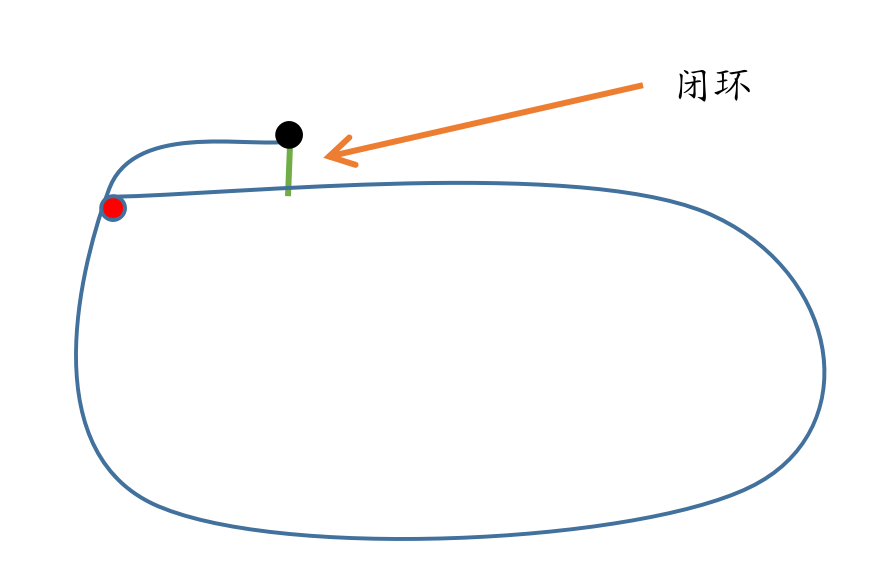
\includegraphics[width=0.4\linewidth]{image/ORB-SLAM/DetectedLoop.png}  %插入的图,包括JPG,PNG,PDF,EPS等,放在源文件目录下
	\caption{检测闭环成功.红点代表起始位置,黑点代表终止位置,绿线代表两张图像相似.}  %图片的名称
	\label{fig:detected_loop}   %标签,用作引用
\end{figure}



图\ref{fig:detected_loop}是闭环检测成功之后的示意图。检测到闭环之后,我们就可以利用闭环关键帧的位姿(累积误差小)来计算得到当前关键帧的位姿,从而减少当前关键帧位姿的累积误差。\textbf{首先},我们要做的就是计算当前关键帧和闭环关键帧之间的Sim3变换(通过对齐两帧之间的3D点得到)。\textbf{然后},由于当前关键帧的点云和闭环关键帧的点云之间相差一个Sim3变换,那么当前关键帧的位姿和闭环关键帧之间的位姿也是相差该Sim3变换(\textbf{note}:想一想3D-3D点对应是如何求位姿的),根据这个原理就能对当前关键帧的位姿进行修复,相当于使用闭环关键帧的位姿计算得到当前关键帧的位姿,从而减少了累积误差。

具体对当前关键帧的位姿进行修复的公式如下:

\begin{equation}
	mg2oScw = gScm * gSmw
\end{equation}
其中,$mg2oScw$表示当前关键帧修复后的位姿,$gScm$表示闭环关键帧到当前关键帧的相对变换Sim3,$gSmw$表示闭环关键帧的绝对位姿(世界坐标系到闭环帧坐标系的变换。该公式就是利用了闭环关键帧的位姿(误差小)计算得到了当前关键帧的位姿,从而减少了当前关键帧位姿的累积误差。


\begin{figure}[h]%%图
	\centering  %插入的图片居中表示
	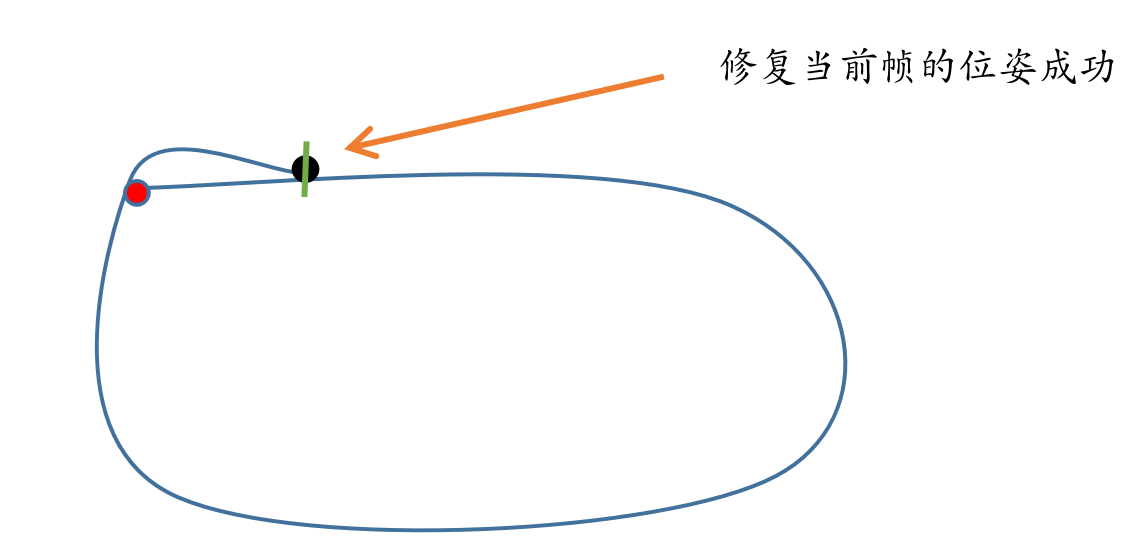
\includegraphics[width=0.5\linewidth]{image/ORB-SLAM/LoopFix1.png}  %插入的图,包括JPG,PNG,PDF,EPS等,放在源文件目录下
	\caption{修复当前关键帧位姿成功.}  %图片的名称
	\label{fig:loop_fix1}   %标签,用作引用
\end{figure}


图\ref{fig:loop_fix1}是当前关键帧对位姿进行修复后的示意图。可见,单单修复当前关键帧的位姿是不行的,还需要修复整个环上其它关键帧的位姿。\textbf{首先},从修复当前关键帧的相邻关键帧(共视关键帧)开始,因为当前关键帧的相邻关键帧是能够看到相同3D点的关键帧,那么当前关键帧通过和闭环关键帧对齐3D点得到的Sim3也是能够用到相邻关键帧上的,那么就也对相邻关键帧的位姿进行了修复。



对当前关键帧的相邻关键帧的位姿进行修复的公式如下:


\begin{equation}
\begin{split}
g2oCorrectedSiw& = g2oSic * mg2oScw \\
&=  g2oSic * gScm * gSmw
\end{split}
\end{equation}

其中,$g2oSic$表示当前关键帧到其第i个相邻关键帧的相对位姿,$mg2oScw$表示当前关键帧修复后的位姿。




\begin{figure}[h]%%图
	\centering  %插入的图片居中表示
	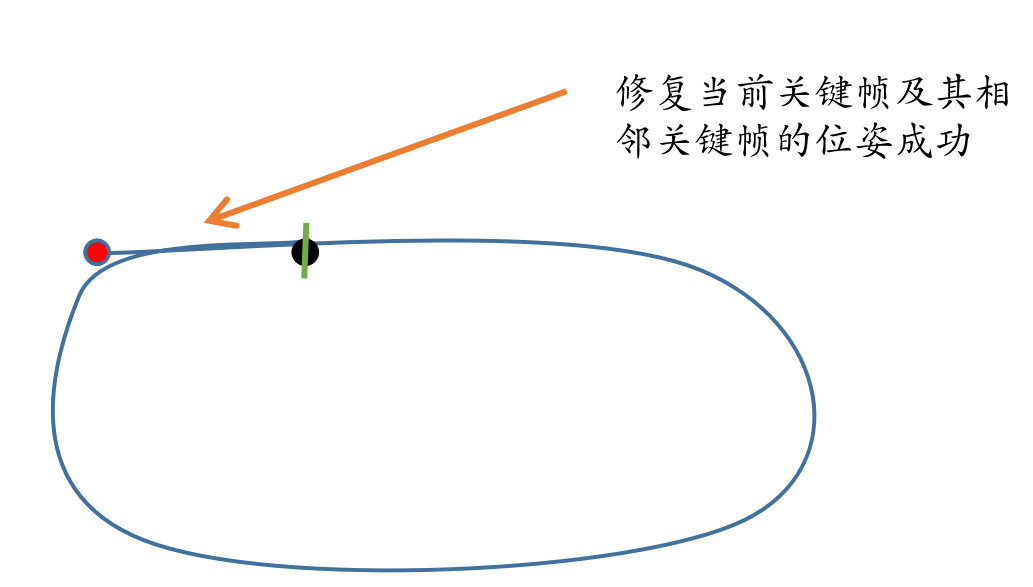
\includegraphics[width=0.5\linewidth]{image/ORB-SLAM/LoopFix2.png}  %插入的图,包括JPG,PNG,PDF,EPS等,放在源文件目录下
	\caption{修复当前关键帧及其相邻关键帧位姿成功.}  %图片的名称
	\label{fig:loop_fix2}   %标签,用作引用
\end{figure}


图\ref{fig:loop_fix2}是修复当前关键帧及其相邻关键帧位姿成功之后的示意图。到此,已经修复了当前关键帧及其相邻关键帧的位姿。但是,如果仅仅修复这些关键帧的位姿的话,没有修复剩余的帧的话,那么就会造成不一致(哪里不一致?),所以就要对剩余的位姿进行修复。而这些关键帧位姿的修复就交给了pose graph optimization。当然了,只要能够最小化整体的误差,pose graph optimization时也会对当前关键帧及其相邻关键帧的位姿进行调整。

那么就下来就是要构造pose grpah了,那么ORB-SLAM2是如何构造pose graph的呢?ORB-SLAM2对所有的关键帧构造一个pose graph,然后对其进行优化。

\textbf{构造顶点},pose graph的顶点(待优化变量)为关键帧的绝对位姿,对于当前关键帧及其相邻关键帧,其绝对位姿就是修复过后的位姿;而对于其它关键帧,其位姿就是原来的位姿;并且优化时,闭环关键帧的位姿被设置为不变,只作为约束条件。

\textbf{构造边},pose graph的边(约束条件)为关键帧之间的相对位姿,那么ORB-SLAM2往pose graph中插入了哪些边呢?

\begin{itemize}
	\item 当前关键帧及其相邻关键帧之间的相对位姿,如图\ref{fig:more_loop_constarint}所示;
	\item 每个关键帧与父亲之间的相对位姿;
	\item 每个关键帧与其回环边之间的相对位姿(不是每个关键帧都有回环边的),每次pose graph optimization之后,都会在当前关键帧和闭环关键帧之间添加一条双向的边。每次进行pose graph optimization时,都会将之前pose graph optimization时生成的回环边加入进来;
	\item 每个关键帧及其相邻关键帧之间的相对位姿。
\end{itemize}

\begin{figure}[h]%%图
	\centering  %插入的图片居中表示
	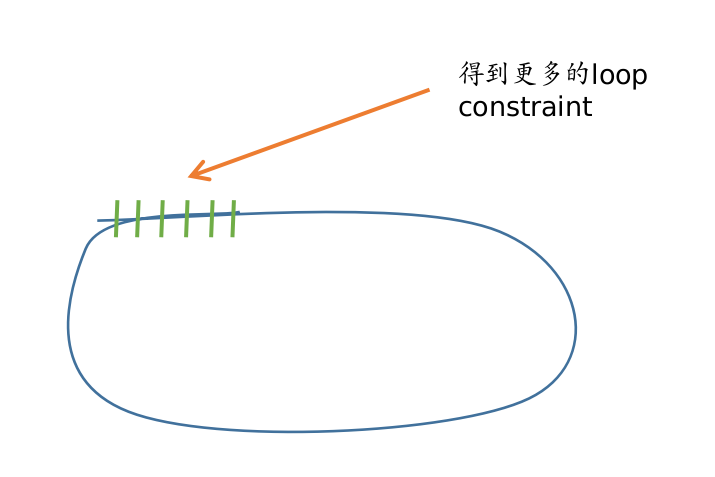
\includegraphics[width=0.5\linewidth]{image/ORB-SLAM/MoreLoopConstraint.png}  %插入的图,包括JPG,PNG,PDF,EPS等,放在源文件目录下
	\caption{当前关键帧及其相邻关键帧的loop constraint.}  %图片的名称
	\label{fig:more_loop_constarint}   %标签,用作引用
\end{figure}

如何ORB-SLAM2是如何计算这些相对位姿(约束条件)的呢?如图\ref{fig:loop_constraint}所示。为什么有时使用\textbf{修复后}的位姿计算相对位姿,有时使用\textbf{修复前}的位姿计算相对位姿呢?

对于第一种情况,使用修复后的位姿计算相对位姿很好理解,因为闭环关键帧及其周围帧的位姿被认为是正确的,那么通过它们修复的当前关键帧及其相邻关键帧的位姿也是正确的,那么它们之间的相对位姿,自然是使用修复过后的位姿进行计算;

至于后面的三种情况,试想一下,如果边的一边是修复后的位姿(当前关键帧或其相邻关键帧的位姿),一边是没有修复的位姿态(除了当前关键帧及其相邻关键帧之外的帧的位姿),那么计算得到的相对位姿肯定是错的,所以要使用\textbf{未修复}之前的位姿来计算相对位姿,通过该约束,从而对边的另一边未修复的位姿进行优化。

\begin{figure}[h]%%图
	\centering  %插入的图片居中表示
	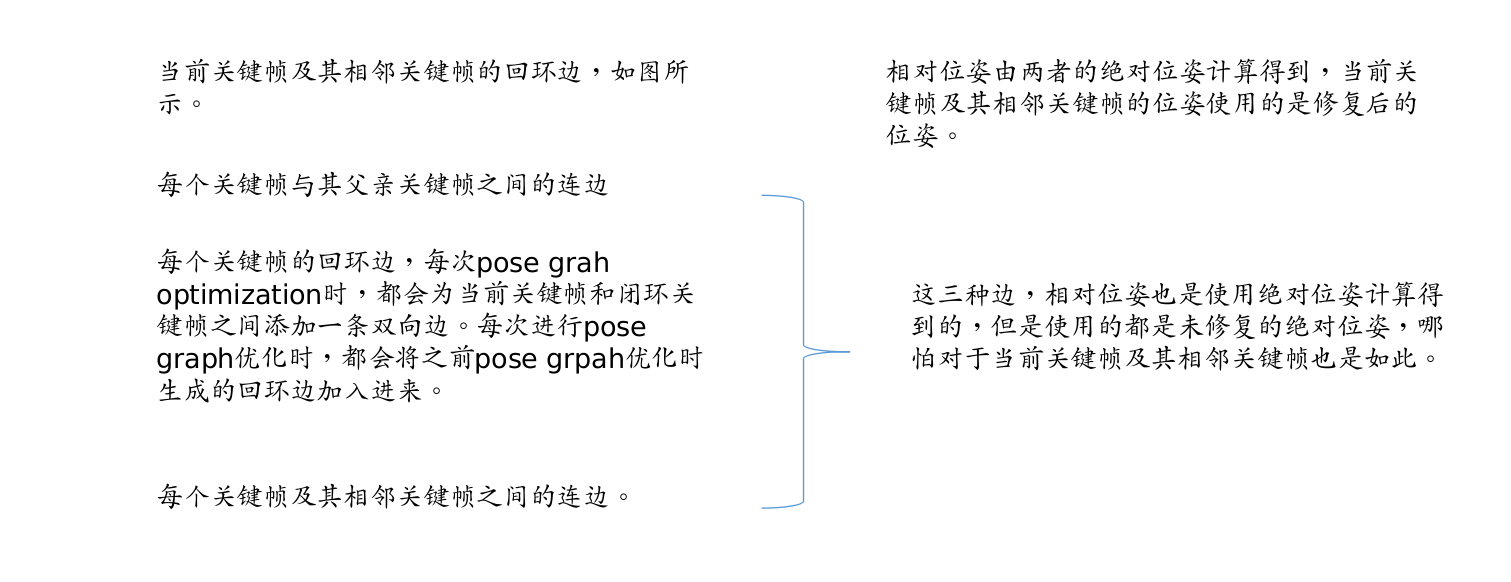
\includegraphics[width=1.0\linewidth]{image/ORB-SLAM/LoopConstraint.png}  %插入的图,包括JPG,PNG,PDF,EPS等,放在源文件目录下
	\caption{ORB-SLAM2如何计算相对位姿.}  %图片的名称
	\label{fig:loop_constraint}   %标签,用作引用
\end{figure}


\begin{note}
	对于pose graph optimization,其成立的基础是相对位姿是准的,但是ORB-SLAM2中的相对位姿是通过绝对位姿计算得到的,既然绝对位姿都是不准的,那么通过其计算得到的相对位姿能是准的吗???
\end{note}


\textbf{姑且认为相对位姿是准的吧},pose graph以相对位姿作用约束,通过优化绝对位姿,减少了误差,并且误差分布到了整个pose graph的顶点上,所以通过pose graph优化后,SLAM的效果能够好很多。但是pose graph优化的前提是检测到闭环,如果SLAM一直前进,不会回到原来走过的地方,那么pose graph也没什么办法。



下面完整地介绍下闭环处理的流程:
\begin{enumerate}
	\item Loop detection
	\item Loop closing
	\item Loop correction
\end{enumerate}

Loop detection就是判断当前走过的地方是不是之前走过的,如果之前就走过了,那么就产生了闭环;Loop closing则是通过闭环关键帧计算得到当前关键帧的位姿,从而减少当前关键帧的累积误差;而Loop correction则是使用pose graph optimization,将闭环得到的信息传播给其它的关键帧,从而减少了其它关键帧的累积误差。



在进行pose graph optimization之后,就要对3D点的位置进行修正。首先,对于每个3D点得到其reference keyframe,也就是哪个关键帧创建了该3D点;然后使用该帧旧的位姿将该3D点转换到该关键帧的坐标系下,然后再使用优化过后的位姿将3D点反投影回到世界坐标系,那么就得到了\textbf{修正}过后的3D点坐标。

在使用pose graph对位姿进行优化,以及使用优化过后的位姿对3D点的坐标进行修正后,LoopClosing线程最后会调用GlobalBundleAdjustment对位姿和3D点进行联合优化。



\section{总结}
ORB-SLAM2中重要的模块差不多就是\textbf{特征点提取}、\textbf{初始化}、\textbf{跟踪}(求下一帧图像的位姿)、\textbf{建图}、\textbf{回环检测}、\textbf{优化}。

\textbf{特征点提取}。对每帧图像提取ORB特征点,并在OpenCV的ORB特征提取的基础上进行改进,使其提取出来的特征在图像上的分布更加均匀。

\textbf{初始化}。单目相机和双目/深度相机的初始化是不同的。双目/深度由于自带深度,所以只需要一帧(对于双目相机来说,这里说的一帧表示同一时刻拍摄的左右帧)就能够完成初始化。而对于单目相机而言,由于缺少了深度相机,所以需要两帧图像才能够完成初始化,单目相机初始化时,需要通过分解\textbf{单应矩阵}H或\textbf{本质矩阵}E来得到位姿,并且通过该位姿对2D-2D特征点对应进行三角测量得到3D点,从而完成单目相机的初始化。

\textbf{跟踪}。跟踪就是不断求下一帧图像位姿的过程。对于SFM来说,一般来说都是通过与一帧图像进行匹配得到2D-2D点对应,并根据传递性,从而得到2D-3D点对应,接着使用PnP来求解位姿。而对于ORB-SLAM2来说,也是通过传递性找到2D-3D点对应,但是ORB-SLAM2并没有使用PnP来求解位姿,而是通过最小化误差来得到下一帧图像的位姿的。对于单目相机,最小化的是重投影误差,对于双目/深度相机,最小化的是立体特征$(u_L, v_L, u_R)$的误差?

\textbf{关键帧选取}。这个判断的条件那是相当复杂,需要看代码才能懂ORB-SLAM2是如何选取关键帧的。不过简单地说的话,就是相距当前关键帧相机移动了一定的距离才需要添加,不过ORB-SLAM2判断的不是距离,而是通过各种2D、3D点的数量来判断相机移动远了,也即是否需要添加关键帧。

\textbf{建图}。跟踪部分对每一帧图像都进行跟踪,而建图则只对那些被选为关键帧的图像帧进行建图。跟踪部分是最小化2D-3D点对应的重投影误差来得到下一帧的位姿的,但是此时下一帧中某些2D点是没有3D点对应的,我们要恢复这部分2D点所对应的3D点,也就是叫做建图了。下一帧关键帧根据Covisibility Graph找到与其相邻的图像帧,并寻找2D-2D点匹配,然后通过三角测量得到新的3D点。

\textbf{回环检测}。回环检测就是通过检测到SLAM过程中是否来到之前已经走过的地方,通过之前帧的位姿来计算当前帧的位姿,从而减少当前帧位姿的累积误差,并且也重新计算当前帧相邻帧的位姿,也减少了这些相邻帧的累积误差。之后,将这个信息传播到整个pose graph上,通过优化pose graph,将累积误差减少的同时,将误差分布到整个pose graph时,从而使得整个SLAM的结果更好。当然,pose graph优化的弊端是必须经过相同的地方,如果SLAM过程中一直往前走,那么pose graph的效果并不会很好。

\textbf{优化}。优化部分包含LocalBundleAdjustment、OptimizeEssentialGraph以及GlobalBundleAdjustment。LocalBundleAdjustment会在局部建图之后,LocalMapping线程空闲时才会调用(没有关键帧需要建图)。OptimizeEssentialGraph就是用在了回环检测上。而GlobalBundleAdjustment之后再纠正闭环之后才会调用。



\section{参考文献}

【AR实验室】mulberryAR:并行提取ORB特征
https://www.cnblogs.com/polobymulberry/p/6270399.html


[ORB-SLAM2] ORB特征提取策略对ORB-SLAM2性能的影响
https://zhuanlan.zhihu.com/p/57235987


[ORB-SLAM2]卡方分布(Chi-squared)外点(outlier)剔除
https://zhuanlan.zhihu.com/p/58556978

orbslam作者的ppt
https://blog.csdn.net/u012700322/article/details/51965152

ORB\_SLAM2中的Sim3优化
https://zhehangt.github.io/2018/11/01/SLAM/ORBSLAM/ORBSLAM2LoopClosingRefine/


ORB-SLAM2从理论到代码实现(五):ORBmatcher.cc程序详解
https://blog.csdn.net/qq\_20123207/article/details/82502207

Loop Closing 3d Point Clouds
https://stackoverflow.com/questions/37279020/loop-closing-3d-point-clouds


ORB-SLAM(十)LoopClosing Sim3求解
https://www.cnblogs.com/shang-slam/p/6480863.html


Scale Drift Issue \#71
https://github.com/raulmur/ORB\_SLAM2/issues/71


